\section{Ejercicio D - Error de la aproximación}

\subsection{Problema}

Recoja en una tabla de datos los puntos $x_i \in [0, 5]$ utilizados en la aproximación numérica de las integrales de Fresnel cuando se utiliza la cuadratura gaussiana de 64 puntos del apartado c) y los $x_i$ necesarios para la aproximación dada en el apartado a), cuando se utiliza la regla compuesta del trapecio con n = 64. (Si prefiere, además de la tabla de datos puede realizar una representación gráfica). Calcule los errores cometidos con estos dos métodos en relación a las estimaciones más exactas de las integrales, es decir, las obtenidas con la extrapolación de Romberg en el apartado b. Discuta los resultados.

\subsection{Resolución}


El código que resuelve el ejercicio se puede ver en \ref{code:ex4}. 

\subsubsection{Puntos $x_i$}

La tabla de puntos se puede ver en \ref{ex4:table}. Una figura de los puntos $x_i$ se puede ver a continuación. 

\begin{figure}[h!]
	\centering
	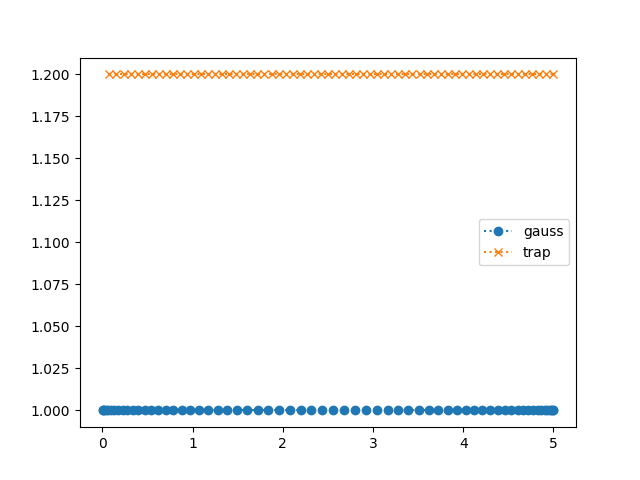
\includegraphics[width=0.8\linewidth]{figures/gauss_trap_xi.png}
	\caption{Gráfica los puntos $x_i$ de la aproximación de Caudratura de Gauss y Regla Compuesta del Trapecio.}
	\label{fig:gauss_trap_xi}
\end{figure}

\paragraph{Discusión} 
La principal diferencia entre los dos conjuntos de $x_i$ es que en el caso de la regla compuesta del trapecio se particiona el intervalo de forma uniforme, mientras que en la cuadratura gaussiana los puntos tienen mayor densidad en los extremos del intervalo.

Esto queda ilustrado muy claramente en la siguiente figura:
\begin{figure}[h!]
	\centering
	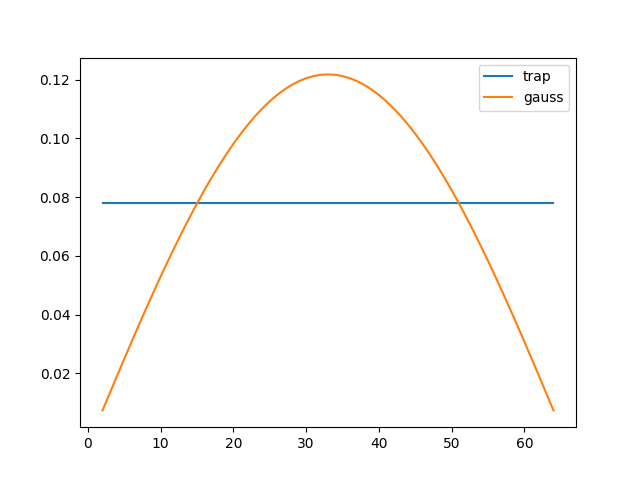
\includegraphics[width=0.8\linewidth]{figures/gauss_trap_diff_xi.png}
	\caption{Diferencia entre los puntos $x_i - x_{i-1}$ de las dos aproximaciones.}
	\label{fig:gauss_trap_diff_xi}
\end{figure}

\subsubsection{Errores}

El error absoluto $v_{approx} - v_{romberg}$ en las aproximaciones, con respecto al valor dado usando el método de Romberg es: 

\begin{table}[H]
	\csvreader[
	tabular=|c|l|l|,
	table head=\hline \textbf{fn} & \textbf{C($\omega$)} & \textbf{S($\omega$)} \\\hline,
	late after last line=\\\hline,
	]{data/abs_error_approx.csv}{}{\csvlinetotablerow}
\end{table}

Y el error relativo, dado por $ 100 * \frac{|err_{abs}|}{v_{romberg}}$: 
\begin{table}[H]
	\csvreader[
	tabular=|c|l|l|,
	table head=\hline \textbf{fn} & \textbf{C($\omega$) (en \%)} & \textbf{S($\omega$) (en \%)} \\\hline,
	late after last line=\\\hline,
	]{data/rel_error_approx.csv}{}{\csvlinetotablerow}
\end{table}

\paragraph{Discusión}
Como vemos, de las dos aproximaciones, la aproximación de cuadratura gaussiana tiene menor error que la de la regla compuesta del trapecio, aunque las dos tienen errores bastante aceptables en este caso.